\documentclass[twoside]{book}

% Packages required by doxygen
\usepackage{fixltx2e}
\usepackage{calc}
\usepackage{doxygen}
\usepackage[export]{adjustbox} % also loads graphicx
\usepackage{graphicx}
\usepackage[utf8]{inputenc}
\usepackage{makeidx}
\usepackage{multicol}
\usepackage{multirow}
\PassOptionsToPackage{warn}{textcomp}
\usepackage{textcomp}
\usepackage[nointegrals]{wasysym}
\usepackage[table]{xcolor}

% Font selection
\usepackage[T1]{fontenc}
\usepackage[scaled=.90]{helvet}
\usepackage{courier}
\usepackage{amssymb}
\usepackage{sectsty}
\renewcommand{\familydefault}{\sfdefault}
\allsectionsfont{%
  \fontseries{bc}\selectfont%
  \color{darkgray}%
}
\renewcommand{\DoxyLabelFont}{%
  \fontseries{bc}\selectfont%
  \color{darkgray}%
}
\newcommand{\+}{\discretionary{\mbox{\scriptsize$\hookleftarrow$}}{}{}}

% Page & text layout
\usepackage{geometry}
\geometry{%
  a4paper,%
  top=2.5cm,%
  bottom=2.5cm,%
  left=2.5cm,%
  right=2.5cm%
}
\tolerance=750
\hfuzz=15pt
\hbadness=750
\setlength{\emergencystretch}{15pt}
\setlength{\parindent}{0cm}
\setlength{\parskip}{3ex plus 2ex minus 2ex}
\makeatletter
\renewcommand{\paragraph}{%
  \@startsection{paragraph}{4}{0ex}{-1.0ex}{1.0ex}{%
    \normalfont\normalsize\bfseries\SS@parafont%
  }%
}
\renewcommand{\subparagraph}{%
  \@startsection{subparagraph}{5}{0ex}{-1.0ex}{1.0ex}{%
    \normalfont\normalsize\bfseries\SS@subparafont%
  }%
}
\makeatother

% Headers & footers
\usepackage{fancyhdr}
\pagestyle{fancyplain}
\fancyhead[LE]{\fancyplain{}{\bfseries\thepage}}
\fancyhead[CE]{\fancyplain{}{}}
\fancyhead[RE]{\fancyplain{}{\bfseries\leftmark}}
\fancyhead[LO]{\fancyplain{}{\bfseries\rightmark}}
\fancyhead[CO]{\fancyplain{}{}}
\fancyhead[RO]{\fancyplain{}{\bfseries\thepage}}
\fancyfoot[LE]{\fancyplain{}{}}
\fancyfoot[CE]{\fancyplain{}{}}
\fancyfoot[RE]{\fancyplain{}{\bfseries\scriptsize Generated by Doxygen }}
\fancyfoot[LO]{\fancyplain{}{\bfseries\scriptsize Generated by Doxygen }}
\fancyfoot[CO]{\fancyplain{}{}}
\fancyfoot[RO]{\fancyplain{}{}}
\renewcommand{\footrulewidth}{0.4pt}
\renewcommand{\chaptermark}[1]{%
  \markboth{#1}{}%
}
\renewcommand{\sectionmark}[1]{%
  \markright{\thesection\ #1}%
}

% Indices & bibliography
\usepackage{natbib}
\usepackage[titles]{tocloft}
\setcounter{tocdepth}{3}
\setcounter{secnumdepth}{5}
\makeindex

% Hyperlinks (required, but should be loaded last)
\usepackage{ifpdf}
\ifpdf
  \usepackage[pdftex,pagebackref=true]{hyperref}
\else
  \usepackage[ps2pdf,pagebackref=true]{hyperref}
\fi
\hypersetup{%
  colorlinks=true,%
  linkcolor=blue,%
  citecolor=blue,%
  unicode%
}

% Custom commands
\newcommand{\clearemptydoublepage}{%
  \newpage{\pagestyle{empty}\cleardoublepage}%
}

\usepackage{caption}
\captionsetup{labelsep=space,justification=centering,font={bf},singlelinecheck=off,skip=4pt,position=top}

%===== C O N T E N T S =====

\begin{document}

% Titlepage & ToC
\hypersetup{pageanchor=false,
             bookmarksnumbered=true,
             pdfencoding=unicode
            }
\pagenumbering{roman}
\begin{titlepage}
\vspace*{7cm}
\begin{center}%
{\Large My Project }\\
\vspace*{1cm}
{\large Generated by Doxygen 1.8.11}\\
\end{center}
\end{titlepage}
\clearemptydoublepage
\tableofcontents
\clearemptydoublepage
\pagenumbering{arabic}
\hypersetup{pageanchor=true}

%--- Begin generated contents ---
\chapter{Hierarchical Index}
\section{Class Hierarchy}
This inheritance list is sorted roughly, but not completely, alphabetically\+:\begin{DoxyCompactList}
\item Http\+Servlet\begin{DoxyCompactList}
\item \contentsline{section}{com.\+ahmet.\+My\+Servlet}{\pageref{classcom_1_1ahmet_1_1_my_servlet}}{}
\end{DoxyCompactList}
\end{DoxyCompactList}

\chapter{Class Index}
\section{Class List}
Here are the classes, structs, unions and interfaces with brief descriptions\+:\begin{DoxyCompactList}
\item\contentsline{section}{\hyperlink{classmain_1_1java_1_1com_1_1ezgi_1_1_ezgis_servlet}{main.\+java.\+com.\+ezgi.\+Ezgis\+Servlet} }{\pageref{classmain_1_1java_1_1com_1_1ezgi_1_1_ezgis_servlet}}{}
\item\contentsline{section}{\hyperlink{classmain_1_1java_1_1com_1_1ezgi_1_1_my_x_m_l_parser}{main.\+java.\+com.\+ezgi.\+My\+X\+M\+L\+Parser} }{\pageref{classmain_1_1java_1_1com_1_1ezgi_1_1_my_x_m_l_parser}}{}
\end{DoxyCompactList}

\chapter{Class Documentation}
\hypertarget{classcom_1_1ahmet_1_1_my_servlet}{}\section{com.\+ahmet.\+My\+Servlet Class Reference}
\label{classcom_1_1ahmet_1_1_my_servlet}\index{com.\+ahmet.\+My\+Servlet@{com.\+ahmet.\+My\+Servlet}}
Inheritance diagram for com.\+ahmet.\+My\+Servlet\+:\begin{figure}[H]
\begin{center}
\leavevmode
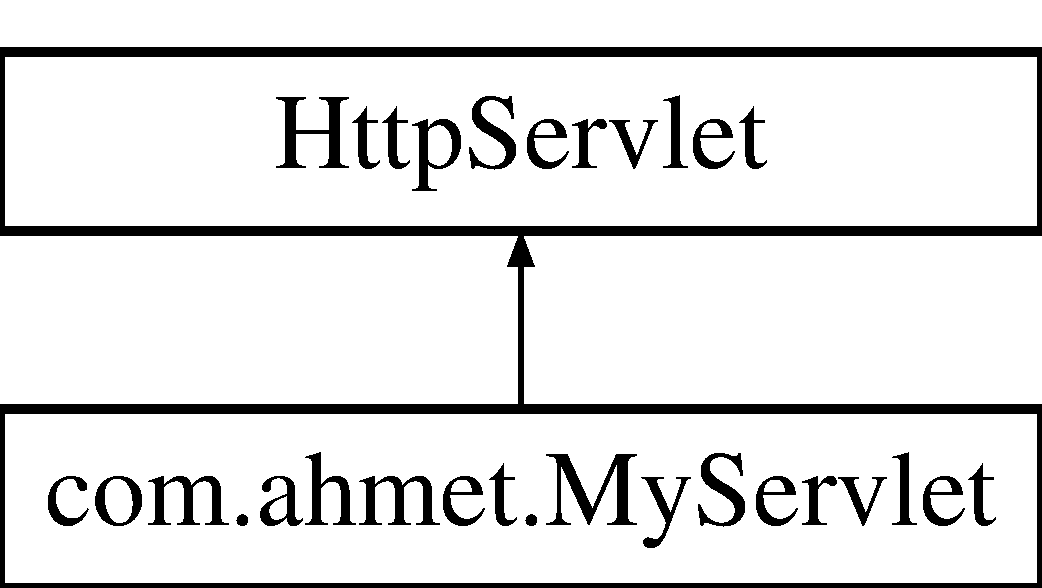
\includegraphics[height=2.000000cm]{classcom_1_1ahmet_1_1_my_servlet}
\end{center}
\end{figure}
\subsection*{Protected Member Functions}
\begin{DoxyCompactItemize}
\item 
void {\bfseries do\+Post} (Http\+Servlet\+Request request, Http\+Servlet\+Response response)  throws Servlet\+Exception, I\+O\+Exception \hypertarget{classcom_1_1ahmet_1_1_my_servlet_ab8741db8d9ad6616215b2a721aff4306}{}\label{classcom_1_1ahmet_1_1_my_servlet_ab8741db8d9ad6616215b2a721aff4306}

\item 
void {\bfseries do\+Get} (Http\+Servlet\+Request request, Http\+Servlet\+Response response)  throws Servlet\+Exception, I\+O\+Exception \hypertarget{classcom_1_1ahmet_1_1_my_servlet_a912a8f77a78c9d08b8df1bbd3e4a20ec}{}\label{classcom_1_1ahmet_1_1_my_servlet_a912a8f77a78c9d08b8df1bbd3e4a20ec}

\end{DoxyCompactItemize}


\subsection{Detailed Description}
Created by Ahmet Ercan Tekden on 20.\+04.\+2016. 

The documentation for this class was generated from the following file\+:\begin{DoxyCompactItemize}
\item 
D\+:/\+Github/bounswe2016group12/\+W\+E\+B\+\_\+\+A\+P\+P/\+Ahmet/src/main/java/com/ahmet/My\+Servlet.\+java\end{DoxyCompactItemize}

\hypertarget{classcom_1_1ahmet_1_1_query_data}{}\section{com.\+ahmet.\+Query\+Data Class Reference}
\label{classcom_1_1ahmet_1_1_query_data}\index{com.\+ahmet.\+Query\+Data@{com.\+ahmet.\+Query\+Data}}
\subsection*{Public Member Functions}
\begin{DoxyCompactItemize}
\item 
\hyperlink{classcom_1_1ahmet_1_1_query_data_a63caeb1484ec80010eea5bf0ae740c1b}{Query\+Data} (String U\+RL)
\item 
void \hyperlink{classcom_1_1ahmet_1_1_query_data_a0148e5b827ac56ac85363d9e1f37cad5}{process\+X\+ML} (String U\+RL)
\item 
int \hyperlink{classcom_1_1ahmet_1_1_query_data_abf5364392a97960a7d008f795ec019ad}{calculate\+Points\+Ahmet} (String query)
\item 
String \hyperlink{classcom_1_1ahmet_1_1_query_data_afa904fbc0828256264eb3b9d55c09354}{get\+U\+R\+L\+Content} (String p\+\_\+s\+U\+RL)
\end{DoxyCompactItemize}


\subsection{Detailed Description}
Created by Ahmet Ercan Tekden on 3.\+05.\+2016. 

\subsection{Constructor \& Destructor Documentation}
\index{com\+::ahmet\+::\+Query\+Data@{com\+::ahmet\+::\+Query\+Data}!Query\+Data@{Query\+Data}}
\index{Query\+Data@{Query\+Data}!com\+::ahmet\+::\+Query\+Data@{com\+::ahmet\+::\+Query\+Data}}
\subsubsection[{\texorpdfstring{Query\+Data(\+String U\+R\+L)}{QueryData(String URL)}}]{\setlength{\rightskip}{0pt plus 5cm}com.\+ahmet.\+Query\+Data.\+Query\+Data (
\begin{DoxyParamCaption}
\item[{String}]{U\+RL}
\end{DoxyParamCaption}
)}\hypertarget{classcom_1_1ahmet_1_1_query_data_a63caeb1484ec80010eea5bf0ae740c1b}{}\label{classcom_1_1ahmet_1_1_query_data_a63caeb1484ec80010eea5bf0ae740c1b}
Creates a Query Objects by processing xml file acquired by connecting to endpoint of sparql link. 
\begin{DoxyParams}{Parameters}
{\em U\+RL} & Rest Endpoint of query which gives xml file \\
\hline
\end{DoxyParams}


\subsection{Member Function Documentation}
\index{com\+::ahmet\+::\+Query\+Data@{com\+::ahmet\+::\+Query\+Data}!calculate\+Points\+Ahmet@{calculate\+Points\+Ahmet}}
\index{calculate\+Points\+Ahmet@{calculate\+Points\+Ahmet}!com\+::ahmet\+::\+Query\+Data@{com\+::ahmet\+::\+Query\+Data}}
\subsubsection[{\texorpdfstring{calculate\+Points\+Ahmet(\+String query)}{calculatePointsAhmet(String query)}}]{\setlength{\rightskip}{0pt plus 5cm}int com.\+ahmet.\+Query\+Data.\+calculate\+Points\+Ahmet (
\begin{DoxyParamCaption}
\item[{String}]{query}
\end{DoxyParamCaption}
)}\hypertarget{classcom_1_1ahmet_1_1_query_data_abf5364392a97960a7d008f795ec019ad}{}\label{classcom_1_1ahmet_1_1_query_data_abf5364392a97960a7d008f795ec019ad}
Calculates points according to my selected data. This is not generic function, it works with my sparql query.


\begin{DoxyParams}{Parameters}
{\em query} & term entered by user. \\
\hline
\end{DoxyParams}
\begin{DoxyReturn}{Returns}
number of rows corresponding to searched user term. 
\end{DoxyReturn}
\index{com\+::ahmet\+::\+Query\+Data@{com\+::ahmet\+::\+Query\+Data}!get\+U\+R\+L\+Content@{get\+U\+R\+L\+Content}}
\index{get\+U\+R\+L\+Content@{get\+U\+R\+L\+Content}!com\+::ahmet\+::\+Query\+Data@{com\+::ahmet\+::\+Query\+Data}}
\subsubsection[{\texorpdfstring{get\+U\+R\+L\+Content(\+String p\+\_\+s\+U\+R\+L)}{getURLContent(String p_sURL)}}]{\setlength{\rightskip}{0pt plus 5cm}String com.\+ahmet.\+Query\+Data.\+get\+U\+R\+L\+Content (
\begin{DoxyParamCaption}
\item[{String}]{p\+\_\+s\+U\+RL}
\end{DoxyParamCaption}
)}\hypertarget{classcom_1_1ahmet_1_1_query_data_afa904fbc0828256264eb3b9d55c09354}{}\label{classcom_1_1ahmet_1_1_query_data_afa904fbc0828256264eb3b9d55c09354}
Gets Source Code of Url 
\begin{DoxyParams}{Parameters}
{\em p\+\_\+s\+U\+RL} & Url of web address \\
\hline
\end{DoxyParams}
\begin{DoxyReturn}{Returns}
String containing source code. 
\end{DoxyReturn}
\index{com\+::ahmet\+::\+Query\+Data@{com\+::ahmet\+::\+Query\+Data}!process\+X\+ML@{process\+X\+ML}}
\index{process\+X\+ML@{process\+X\+ML}!com\+::ahmet\+::\+Query\+Data@{com\+::ahmet\+::\+Query\+Data}}
\subsubsection[{\texorpdfstring{process\+X\+M\+L(\+String U\+R\+L)}{processXML(String URL)}}]{\setlength{\rightskip}{0pt plus 5cm}void com.\+ahmet.\+Query\+Data.\+process\+X\+ML (
\begin{DoxyParamCaption}
\item[{String}]{U\+RL}
\end{DoxyParamCaption}
)}\hypertarget{classcom_1_1ahmet_1_1_query_data_a0148e5b827ac56ac85363d9e1f37cad5}{}\label{classcom_1_1ahmet_1_1_query_data_a0148e5b827ac56ac85363d9e1f37cad5}
Processes xml of given url to to create table data. 
\begin{DoxyParams}{Parameters}
{\em U\+RL} & Url of Xml of sparql query. \\
\hline
\end{DoxyParams}


The documentation for this class was generated from the following file\+:\begin{DoxyCompactItemize}
\item 
src/main/java/com/ahmet/Query\+Data.\+java\end{DoxyCompactItemize}

\hypertarget{classcom_1_1ahmet_1_1_query_data_test}{}\section{com.\+ahmet.\+Query\+Data\+Test Class Reference}
\label{classcom_1_1ahmet_1_1_query_data_test}\index{com.\+ahmet.\+Query\+Data\+Test@{com.\+ahmet.\+Query\+Data\+Test}}
\subsection*{Public Member Functions}
\begin{DoxyCompactItemize}
\item 
void {\bfseries test\+Column} ()\hypertarget{classcom_1_1ahmet_1_1_query_data_test_aacd06ea409eb7bcaaf88fee8521c73e2}{}\label{classcom_1_1ahmet_1_1_query_data_test_aacd06ea409eb7bcaaf88fee8521c73e2}

\item 
void {\bfseries test\+Row} ()\hypertarget{classcom_1_1ahmet_1_1_query_data_test_a7ac076eaca5768c2c949663864708ce4}{}\label{classcom_1_1ahmet_1_1_query_data_test_a7ac076eaca5768c2c949663864708ce4}

\end{DoxyCompactItemize}
\subsection*{Static Public Member Functions}
\begin{DoxyCompactItemize}
\item 
static void {\bfseries test\+Setup} ()\hypertarget{classcom_1_1ahmet_1_1_query_data_test_aea85bf8914c3849838f67bc791a4e4eb}{}\label{classcom_1_1ahmet_1_1_query_data_test_aea85bf8914c3849838f67bc791a4e4eb}

\end{DoxyCompactItemize}


\subsection{Detailed Description}
Created by Ahmet Ercan Tekden on 6.\+05.\+2016. 

The documentation for this class was generated from the following file\+:\begin{DoxyCompactItemize}
\item 
src/test/java/com/ahmet/Query\+Data\+Test.\+java\end{DoxyCompactItemize}

%--- End generated contents ---

% Index
\backmatter
\newpage
\phantomsection
\clearemptydoublepage
\addcontentsline{toc}{chapter}{Index}
\printindex

\end{document}
